\documentclass[aspectratio=169,handout,bigger]{beamer}

\usepackage{minted}
\usepackage[utf8]{inputenc}
\usepackage{graphicx}
\usepackage[T1,T2A]{fontenc}
\usepackage[american,russian]{babel}

\usepackage{tikz}
\usetikzlibrary{shapes,arrows,chains,calc,fit,matrix}
\tikzstyle{line}=[draw]
\tikzstyle{arrow}=[draw]

%% -------------------------------------------------------------------------- %%

\mode<presentation>{
  \usetheme{default}
}

\setbeamertemplate{navigation symbols}{}
\setbeamertemplate{footline}[frame number]

\newcommand{\comment}[1]{}

%% -------------------------------------------------------------------------- %%

\title{
\includegraphics[height=.15\textheight]{logo}}
\author{Пользовательская автоматизация\newlineпрофессиональных веб-приложений\newlineна Lua}
\institute{Александр Гладыш\newline@agladysh}
\date{\\Рязанский IT Workshop\\Сентябрь 2018}

%% -------------------------------------------------------------------------- %%

\begin{document}

\maketitle

%% -------------------------------------------------------------------------- %%

\section{Задача}

%% -------------------------------------------------------------------------- %%

\begin{frame}{Профессиональные приложения}

Профессиональное приложение:

\begin{itemize}
\item Для профессионалов, глубоко владеющих предметной областью
\item Которые в большинстве своём не айтишники
\end{itemize}

\end{frame}

%% -------------------------------------------------------------------------- %%

\begin{frame}{Конкретика}

\begin{itemize}
\item ТАИС разрабатывает профессиональное ПО для гражданской авиации
\item Глубокая и обширная предметная область с длинной историей
\item Требует профессионального обучения пользователей
\end{itemize}

\end{frame}

%% -------------------------------------------------------------------------- %%

\begin{frame}{Пользовательский интерфейс предыдущего поколения}

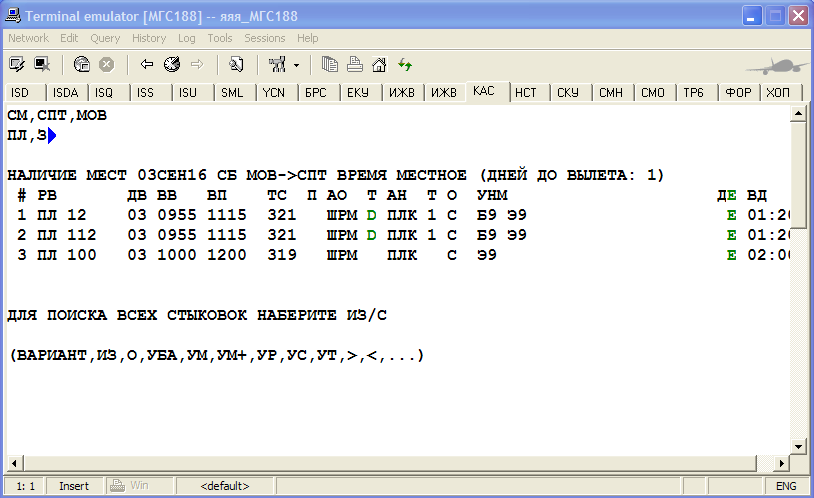
\includegraphics[width=.90\textwidth]{temul}

\end{frame}

%% -------------------------------------------------------------------------- %%

\begin{frame}{Перспективный пользовательский интерфейс}

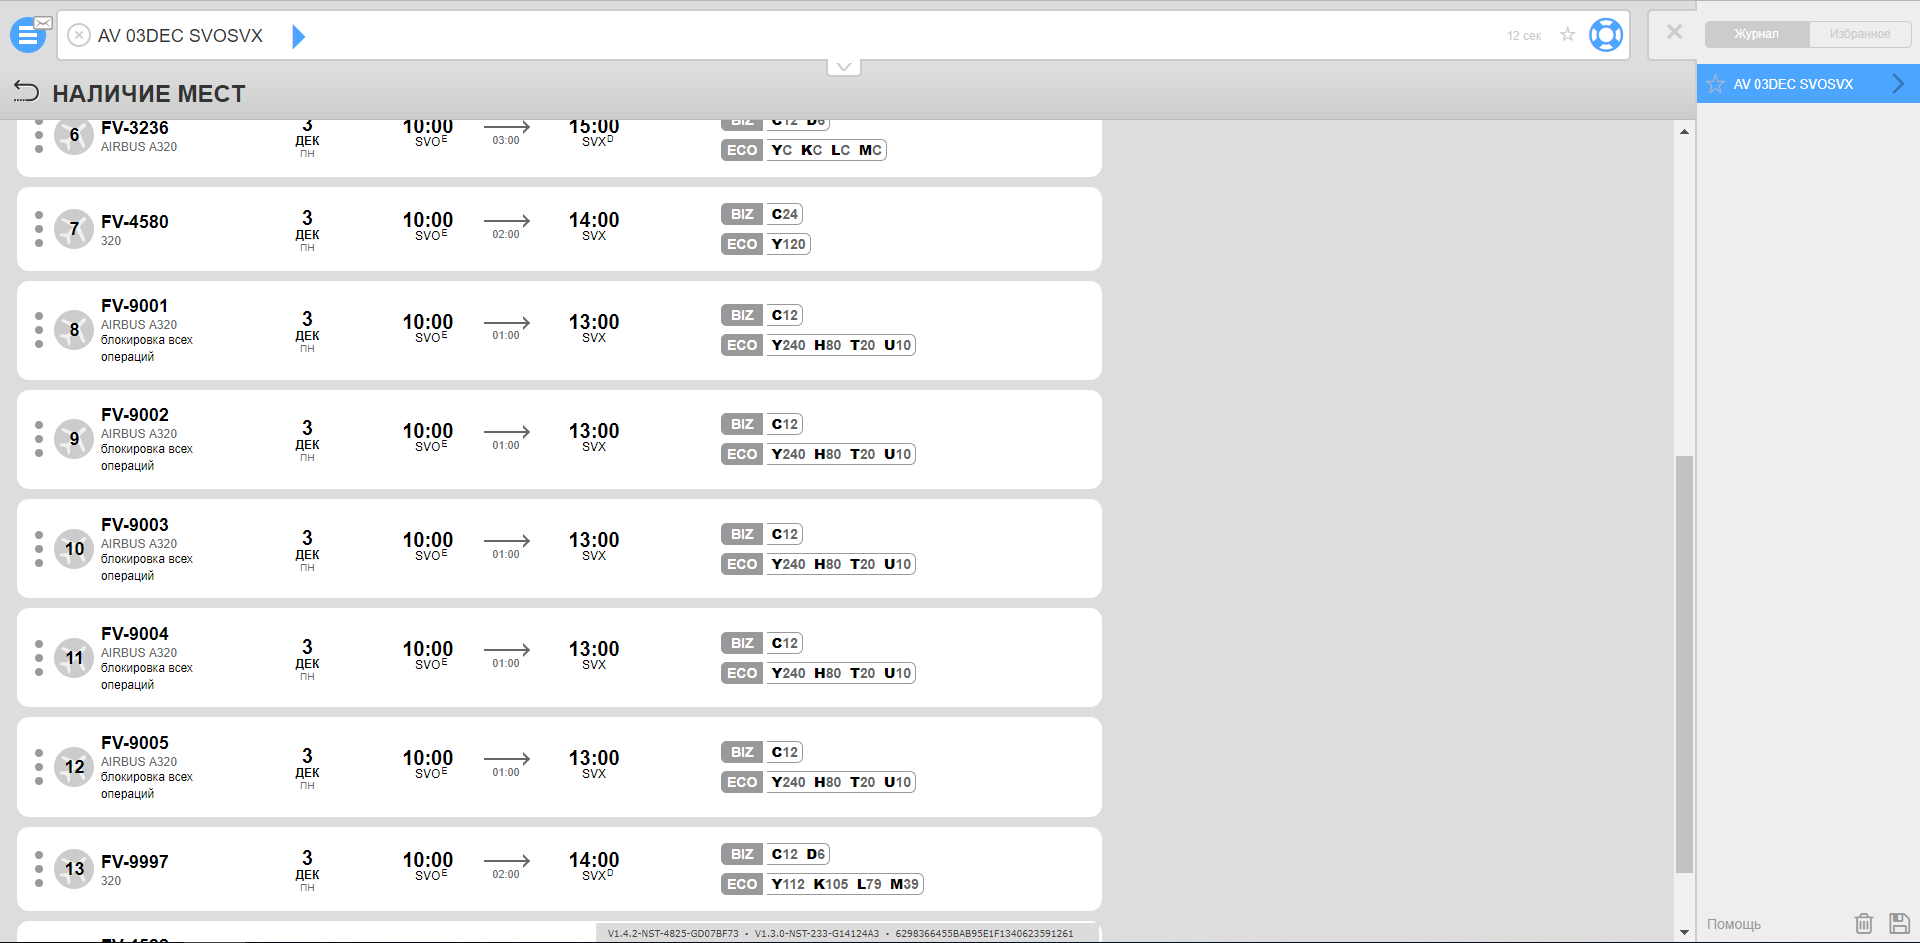
\includegraphics[width=.90\textwidth]{twt}

\end{frame}

%% -------------------------------------------------------------------------- %%

\begin{frame}{Многослойная система}

\begin{tikzpicture}

\node (ui) {Пользовательский интерфейс};
\node (cryptic) [below of=ui] {Прикладные команды ("Криптик")};
\node (app) [below of=cryptic] {Веб-приложение};
\node (browser) [below of=app] {Браузер};
\node (server) [below of=browser] {REST-сервер};
\node (crs) [below of=server] {Хост CRS};

\draw [arrow] (ui) -> (cryptic);
\draw [arrow] (cryptic) -> (app);
\draw [arrow] (app) -> (browser);
\draw [arrow] (browser) -> (server);
\draw [arrow] (server) -> (crs);

\end{tikzpicture}

\end{frame}

%% -------------------------------------------------------------------------- %%

\begin{frame}{Задачи}

\begin{itemize}
\item Автоматизация редких но сложных операций пользователя-эксперта
\item В дальнейшем --- удобное API для более широкого круга пользователей
\end{itemize}

\end{frame}

%% -------------------------------------------------------------------------- %%

\section{Решение}

%% -------------------------------------------------------------------------- %%

\begin{frame}{Почему макросы на клиенте?}

\begin{itemize}
\item Запускать код пользователя на сервере — головная боль
\item Особенно если уже есть система пользовательских команд
\item Даже если её нет — у вас же есть серверное HTTP-API, правда?
\end{itemize}

\end{frame}

%% -------------------------------------------------------------------------- %%

\begin{frame}{Многослойная система с макросами}

\begin{tikzpicture}

\node (macro) {Пользовательский интерфейс};
\node (ui) [right= 1cm of macro] {Макросы на Lua};
\node (cryptic) [below of=ui, below of=macro]{Прикладные команды};
\node (app) [below of=cryptic] {Веб-приложение};
\node (browser) [below of=app] {Браузер};
\node (server) [below of=browser] {REST-сервер};
\node (crs) [below of=server] {Хост CRS};

\draw [arrow] (ui) -> (cryptic);
\draw [arrow] (macro) -> (cryptic);
\draw [arrow] (cryptic) -> (app);
\draw [arrow] (app) -> (browser);
\draw [arrow] (browser) -> (server);
\draw [arrow] (server) -> (crs);

\end{tikzpicture}

\end{frame}

%% -------------------------------------------------------------------------- %%

\begin{frame}{Почему Lua?}

\begin{itemize}
\item Lua легче освоить непрограммистам
\item JavaScript тяжело изолировать от "кишок" проекта
\item Lua легко изолировать
\item Сам факт использования другого языка делает дизайн API чище
\end{itemize}

\end{frame}

%% -------------------------------------------------------------------------- %%

\begin{frame}{Внешний вид: редактор скриптов}

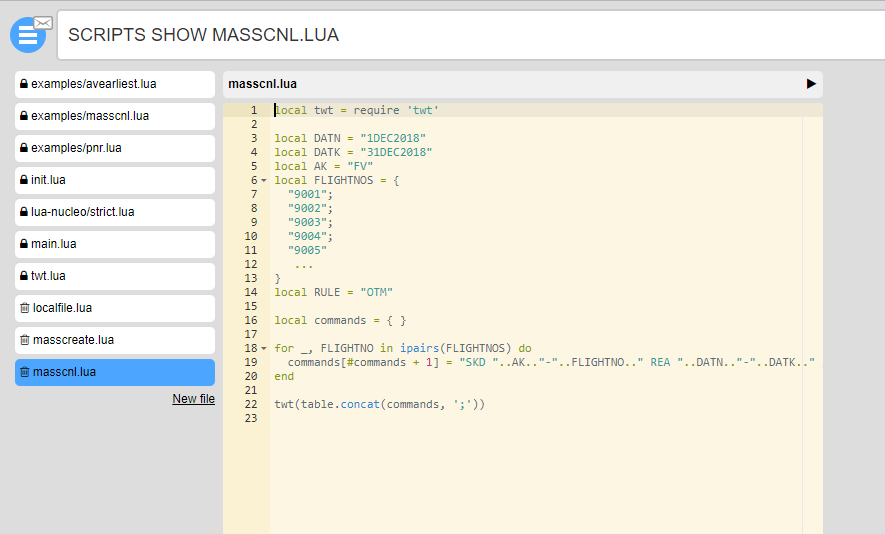
\includegraphics[width=.90\textwidth]{scripts}

\end{frame}

%% -------------------------------------------------------------------------- %%

\begin{frame}{Внешний вид: результат выполнения}

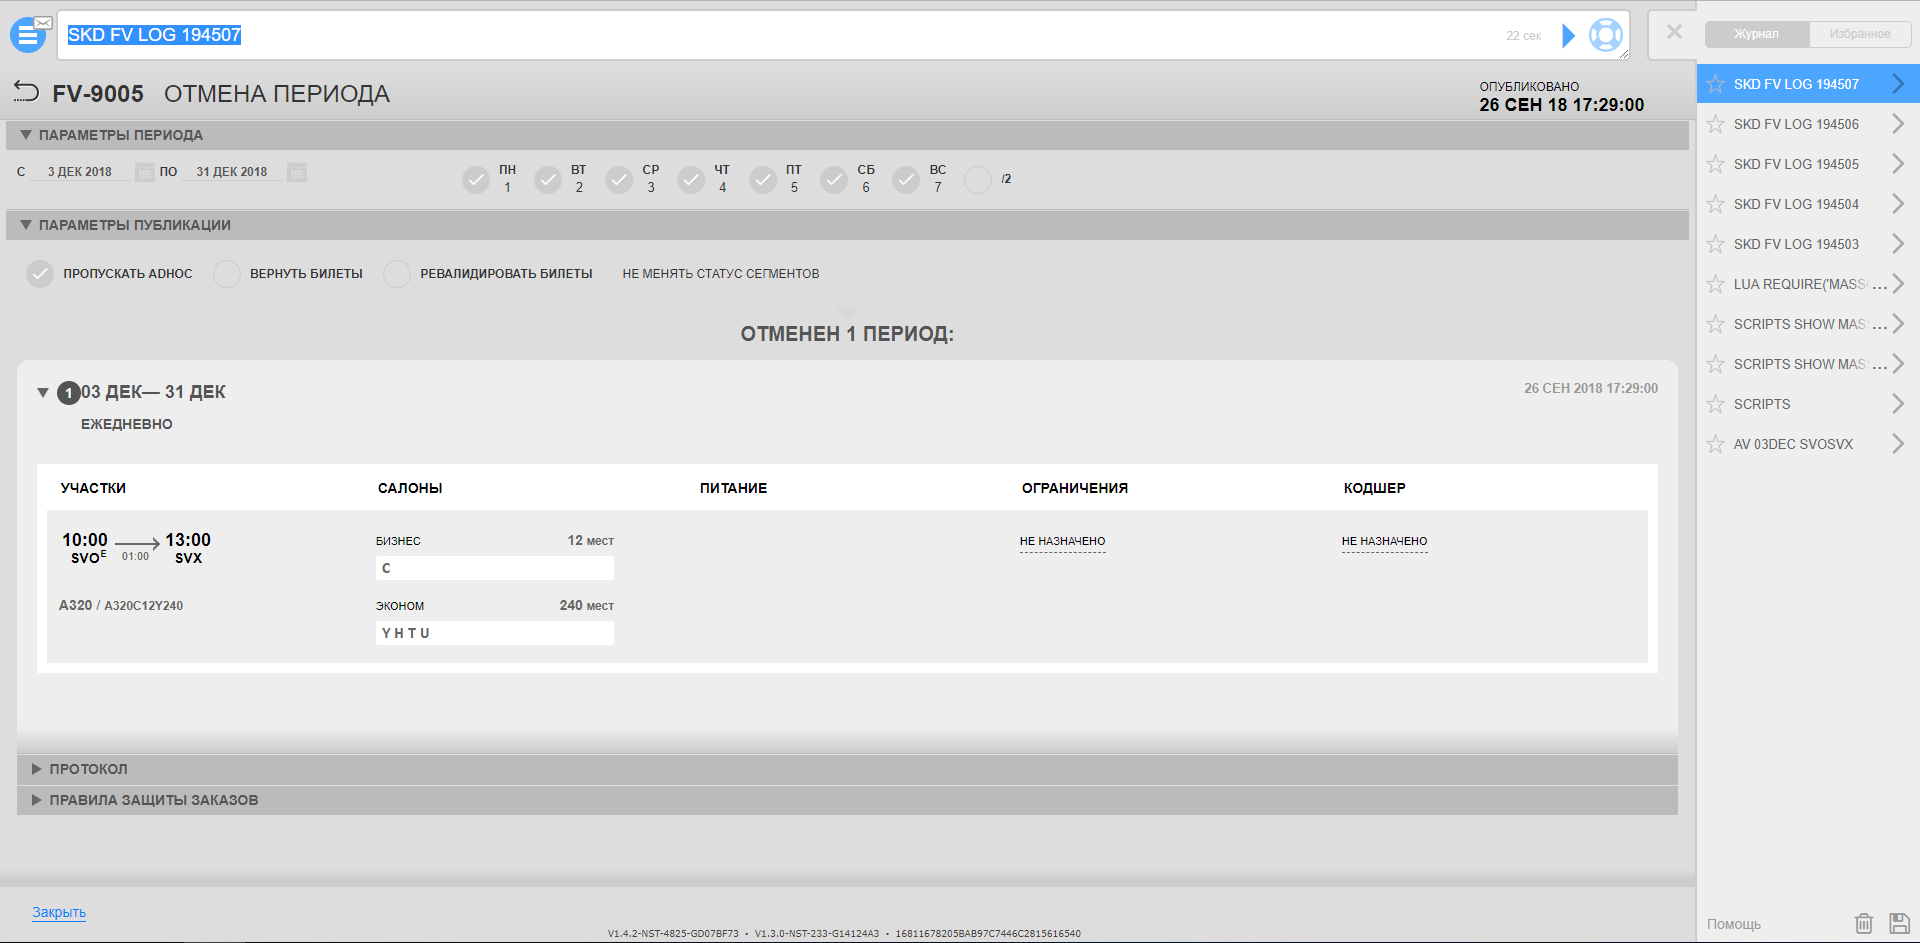
\includegraphics[width=.90\textwidth]{result}

\end{frame}

%% -------------------------------------------------------------------------- %%

\begin{frame}{Lua в браузере: основные варианты}

\begin{itemize}
\item lua.vm.js
\item fengari
\end{itemize}

См. также: Sailor MVC

\end{frame}

%% -------------------------------------------------------------------------- %%

\begin{frame}{Наш стек}

\begin{itemize}
\item lua.vm.js
\item API для выполнения команд и анализа результатов
\item Маленькая самописная библиотека для VFS
\item ACE (brace)
\item webpack
\end{itemize}

\end{frame}

%% -------------------------------------------------------------------------- %%

\begin{frame}[fragile]{Немного кода: Пример макроса}

\begin{minted}{lua}
local twt = require 'twt'

local DATN, DATK = "23JUL2018", "31DEC2018"
local AK, FLIGHTNOS = "R3", { "401"; "756" } -- ...

local commands = { }
for _, FLIGHTNO in ipairs(FLIGHTNOS) do
  -- SKD R3-401 REA 23JUL2018-31DEC2018 !EXEC
  commands[#commands + 1] = "SKD "..AK.."-"..FLIGHTNO
    .." REA "..DATN.."-"..DATK.." !EXEC"
end

twt(table.concat(commands, ';'))
\end{minted}

\end{frame}

%% -------------------------------------------------------------------------- %%

\begin{frame}[fragile]{Немного кода: обёртка над VM}

\begin{minted}{javascript}
var LuaVM = require('lua.vm.js');

var execute = function(code) { return this.lua_.execute(code); };
var provideModule = function(name, value) {
  this.lua_._G.get("package").get("loaded").set(name, value);
};

var Vm = function() { this.lua_ = new LuaVM.Lua.State(); };

Vm.prototype = {
  execute: execute,
  provideModule: provideModule,
  constructor: Vm
};
module.exports = Vm;
\end{minted}

\end{frame}

%% -------------------------------------------------------------------------- %%

\begin{frame}[fragile]{Немного кода: пример модуля Lua на JS}

\begin{minted}{javascript}
vm.provideModule("twt.terminal", {
  alert: function() {
    var msg = this;
    alert("Lua says:\n\n" + msg);
  },

  log: function() {
    var args = (arguments.length === 1)
      ? [ arguments[0] ]
      : Array.apply(null, arguments)
      ;
    args.unshift(this); // First argument passed as this
    log.log.apply(log, args);
  }
});
\end{minted}

\end{frame}

%% -------------------------------------------------------------------------- %%
\begin{frame}[fragile]{Немного кода: запуск Lua}

\begin{minted}{javascript}
vm.execute([
 "assert(loadstring(",
   "assert(require('twt.vfs'):get('init.lua'),
      'missing init.lua'),",
   "'@init.lua'",
 "))()"
].join("\n"));
\end{minted}

\end{frame}

%% -------------------------------------------------------------------------- %%

\begin{frame}[fragile]{Немного кода: init.lua, работа с модулями}

\begin{minted}{lua}
  local vfs = require 'twt.vfs'
  local searchers = package.searchers
  -- Keep package.preload handler intact
  package.searchers = { searchers[1] }
  package.searchers[#package.searchers + 1] = function(filename)
    if not filename:find("%.lua$") then
      filename = filename .. ".lua"
    end
    local file = vfs:get(filename)
    if not file then
      return "\ncan't find the module"
    end
    return assert(loadstring(file, "@" .. filename))
  end
end
\end{minted}

\end{frame}

%% -------------------------------------------------------------------------- %%

\begin{frame}{Что дальше?}

\begin{itemize}
\item Технически — Lua в браузере отлично работает и выполняет свои задачи.
\item Главное — это удобство использования, а это уже вопрос дизайна API.
\end{itemize}

\end{frame}

%% -------------------------------------------------------------------------- %%

\section{Вопросы?}

%% -------------------------------------------------------------------------- %%

\begin{frame}{Вопросы?}

Alexander Gladysh\newline
@agladysh\newline
\newline
t.me/luainmoscow

\end{frame}

%% -------------------------------------------------------------------------- %%

\end{document}

%% -------------------------------------------------------------------------- %%
